%% ----------------------------------------------------------------
%% Introduction | What is VC? How does it work?
%% ---------------------------------------------------------------- 


\begin{quote} 
    \centering 
        "100\% of \textit{NOTHING} is a lot less than 17\% of a \textbf{BIG COMPANY}"\\
    \raggedleft
        \emph{by Anonymous}
\end{quote}

%%%%%%%%%%%%%%%%%%%%%%%%%%%%%%%%%%%%%%%%
%%%%       NEW SECTION              %%%%
%%%%%%%%%%%%%%%%%%%%%%%%%%%%%%%%%%%%%%%%
\section{Rationale of the research}

Venture Capital (VC) firms are financial intermediaries  that provide funding to 'startups', usually these are young and innovative companies working in Software, Biotech and Media \& Entertainment fields.

See \ref{tab:vc_industry} for 2015-2016 by-industry breakdown of VC investments in US.
It is clear that majority of investment consistently goes to Software (vast majority fluctuating around 40\%), Biotech and Media \& Entertainment startups.

If one chooses a less-granular classification, then computer-technology and software-related startups will take an even more dominant position.

Typical setup for a VC deal is as follows:
\begin{itemize}
    \item VC screens thousands of startup applications, invites select few for presentations and starts negotiations
    \item VC invests cash in chosen startups in exchange for:
        \begin{itemize}
            \item share of equity
            \item board seats
            \item control rights
            \item etc...
        \end{itemize}
    \item this creates a 'valuation' described by equation \ref{eq:valuation}
\end{itemize}

\begin{equation}
\label{eq:valuation}
    Valuation = \frac{VC \hspace{0.2cm} investment \hspace{0.2cm} \$}{Equity \hspace{0.2cm} \% \hspace{0.2cm} purchased}
\end{equation}

One should differentiate between different types of VC investment, these are:
\begin{enumerate}
    \item seed stage
    \item early stage
    \item later stage
    \item expansion stage
\end{enumerate}

The line between stages is somewhat blurred and there is no solid consensus on the subject. Nevertheless, for the most classic methodology refer to  figure \ref{fig:fin_cycle}

\begin{figure}[ht]
    \centering
    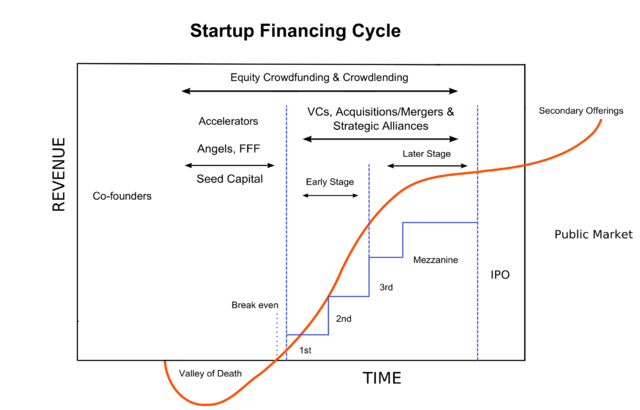
\includegraphics[scale=0.65]{fin_cycle}
    \caption{Startup Financing Cycle\\Source: Public domain}
    \label{fig:fin_cycle}
\end{figure}

Most often VCs invest in \emph{early stage}, as suggested by table \ref{tab:vc_stage_num} with \emph{expansion stage} coming in second, \emph{later stage} being third and \emph{seed stage} receiving the least amount of deals.

This is very illustrative of VCs risk-return preferences, more on this below in this chapter.

At the same time, average investment amount per deal increases as company comes to later stages, since risk decreases if a company has user base, revenues, experience and hasn't failed so far. Therefore it's not surprising that \emph{seed stage} attracts the least amount of cash, while \emph{early, expansion and later stages} receive approximately the same amount of total USD funding, according to table \ref{tab:vc_stage_usd}.

%%-------------------------------------------------------------------------%%
%% Latex Tables Created using http://www.tablesgenerator.com/latex_tables  %%
%%-------------------------------------------------------------------------%%

\begin{table}[!htbp]
    \centering
    \hspace*{-1.5cm}
    \begin{tabular}{rrrrrr}
                        & \textbf{Seed Stage} & \textbf{Early Stage} & \textbf{Expansion Stage} & \textbf{Later Stage} & \textbf{Grand Total} \\ \hline
    \textbf{2012 Total} & 305                 & 1,831                & 1,011                    & 853                  & 4,000                \\ \hline
    \textbf{2013 Total} & 244                 & 2,206                & 1,034                    & 816                  & 4,300                \\ \hline
    \textbf{2014 Total} & 212                 & 2,213                & 1,173                    & 873                  & 4,471                \\ \hline
    \textbf{2015 Total} & 197                 & 2,279                & 1,168                    & 853                  & 4,497                \\ \hline
    \textbf{2016 Q1}    & 62                  & 406                  & 288                      & 213                  & 969                 
    \end{tabular}
\caption{Num. of Deals distribution of VC investments by stages\\Source: \parencite{moneytree}}
\label{tab:vc_stage_num}
\hspace*{-1cm}
\end{table}

\begin{table}[!htbp]
    \hspace*{-1.5cm}
    \centering
    \begin{tabular}{rrrrrr}
    \multicolumn{1}{c}{} & \multicolumn{1}{c}{\textbf{Seed Stage}} & \multicolumn{1}{c}{\textbf{Early Stage}} & \multicolumn{1}{c}{\textbf{Expansion Stage}} & \multicolumn{1}{c}{\textbf{Later Stage}} & \multicolumn{1}{c}{\textbf{Grand Total}} \\ \hline
    \textbf{2011 Total}  & 4\%                                     & 31\%                                     & 33\%                                         & 32\%                                     & 100\%                                    \\ \hline
    \textbf{2012 Total}  & 3\%                                     & 31\%                                     & 35\%                                         & 31\%                                     & 100\%                                    \\ \hline
    \textbf{2013 Total}  & 3\%                                     & 34\%                                     & 33\%                                         & 29\%                                     & 100\%                                    \\ \hline
    \textbf{2014 Total}  & 2\%                                     & 32\%                                     & 42\%                                         & 24\%                                     & 100\%                                    \\ \hline
    \textbf{2015 Total}  & 2\%                                     & 34\%                                     & 37\%                                         & 27\%                                     & 100\%                                    \\ \hline
    \textbf{2016 Q1}  & 3\%                                     & 35\%                                     & 33\%                                         & 29\%                                     & 100\%                                   
    \end{tabular}
    \caption{Money distribution of VC investments by stages\\Source: \parencite{moneytree}, author's calculations}
    \label{tab:vc_stage_usd}
    \hspace*{-1.2cm}
\end{table}





%%-------------------------------------------------------------------------
%% Latex Tables Created using http://www.tablesgenerator.com/latex_tables
%%-------------------------------------------------------------------------

\begin{table}[!htbp]
    
    \hspace*{-1.5cm}
    \begin{tabular}{lrrrr}
        \textbf{Industry}                       & \multicolumn{1}{c}{\textbf{2015 Total}} & \multicolumn{1}{c}{\textbf{2016 q1}} & \multicolumn{1}{c}{\textbf{2015 Total}} & \multicolumn{1}{c}{\textbf{2016q1}} \\ \hline
        \textbf{Software}                       & \$23.67 Bil.                   & \$5.07 Bil.                 & 39.65\%                         & 41.80\%                    \\ \hline
        \textbf{Biotechnology}                  & \$7.72 Bil.                    & \$1.81 Bil.                 & 12.93\%                         & 14.87\%                    \\ \hline
        \textbf{Media and Entertainment}        & \$5.25 Bil.                    & \$0.93 Bil.                 & 8.80\%                          & 7.66\%                     \\ \hline
        \textbf{Consumer Products and Services} & \$4.84 Bil.                    & \$0.23 Bil.                 & 8.11\%                          & 1.89\%                     \\ \hline
        \textbf{IT Services}                    & \$3.89 Bil.                    & \$0.82 Bil.                 & 6.52\%                          & 6.76\%                     \\ \hline
        \textbf{Financial Services}             & \$3.28 Bil.                    & \$0.42 Bil.                 & 5.49\%                          & 3.43\%                     \\ \hline
        \textbf{Industrial/Energy}              & \$3.22 Bil.                    & \$0.64 Bil.                 & 5.40\%                          & 5.24\%                     \\ \hline
        \textbf{Medical Devices and Equipment}  & \$2.8 Bil.                     & \$0.51 Bil.                 & 4.69\%                          & 4.19\%                     \\ \hline
        \textbf{Retailing/Distribution}         & \$1.03 Bil.                    & \$0.09 Bil.                 & 1.73\%                          & 0.74\%                     \\ \hline
        \textbf{Healthcare Services}            & \$0.81 Bil.                    & \$0.13 Bil.                 & 1.36\%                          & 1.08\%                     \\ \hline
        \textbf{Computers and Peripherals}      & \$0.74 Bil.                    & \$0.87 Bil.                 & 1.24\%                          & 7.18\%                     \\ \hline
        \textbf{Semiconductors}                 & \$0.72 Bil.                    & \$0.12 Bil.                 & 1.21\%                          & 0.96\%                     \\ \hline
        \textbf{Telecommunications}             & \$0.72 Bil.                    & \$0.19 Bil.                 & 1.21\%                          & 1.57\%                     \\ \hline
        \textbf{Electronics/Instrumentation}    & \$0.4 Bil.                     & \$0.11 Bil.                 & 0.67\%                          & 0.92\%                     \\ \hline
        \textbf{Networking and Equipment}       & \$0.29 Bil.                    & \$0.09 Bil.                 & 0.49\%                          & 0.76\%                     \\ \hline
        \textbf{Business Products and Services} & \$0.25 Bil.                    & \$0.12 Bil.                 & 0.41\%                          & 0.95\%                     \\ \hline
        \textbf{Other}                          & \$0.06 Bil.                    & \$0 Bil.                    & 0.10\%                          & 0.00\%                     \\ \hline
        \textbf{Total}                          & \$59.7 Bil.                    & \$12.14 Bil.                & 100.00\%                        & 100.00\%                  
    \end{tabular}
    \caption{Total VC investment by Industry \\Source: Data from \parencite{moneytree}, author's calculations}
    \label{tab:vc_industry}
    \hspace*{-1cm}
\end{table}

\newpage


\begin{quote} 
    \centering 
        “The venture capital business is a 100\% game of outliers - it’s extreme exceptions. There are on the order of 4000 'fundable' companies a year, that want to raise venture capital. About 200 of those will get funded by what’s considered a 'top tier VC'; about 15 of those will someday get to a 100M in revenue...and those 15 from that year, will generate something on the order of 97\% of all the returns for the entire category of VC in that year.”\\
    \raggedleft
        \emph{\parencite{anderseen:raise}}
\end{quote}

The nature of VC investments is risky by definition, that explains why funds prefer early stage investments: seed stage startups are often too risky even for VCs, while investing at later stages in more solid startups yields lesser returns due to lower risks. Thus early stage has the optimal risk-return ratio for a VC fund.

To better understand VCs, let's take a look at inner workings of a typical fund.

There is the VC team, i.e. management, and there are (usually) external money which management is ought to invest into startups as they see fit. This money often comes from institutional investors expecting a competitive return on their funds. To achieve this goal, the VC needs overall returns of \%35+ on a horizon of 3 to 5 years.

To achieve this, VC needs to follow several guidelines:
\begin{itemize}
    \item maximise investor revenue to outperform alternative investment vehicles (e.g. low-risk ETFs or risk-free T-Bills)
    \item gain control in funded companies to steer them towards profit and profitable exit \footnote{In VC jargon, an 'exit' is when VC fund liquidates it's shares in the company either via acquisition by some company or an IPO}
    \item have the ability to exit the investment on a satisfactory timescale and return rate
    \item grow reputation to attract promising startups at more favourable conditions
    \item find a sufficient number of promising investment opportunities to invest all available funds
    
\end{itemize}

I will mostly be focusing on US because it is the most mature, well functioning market with the longest history of Venture Capital and public market trading. Also, compared to Europe, IPO financing is much more common in USA, compared to traditional bank and bond financing.

VC is a historically new phenomena, when Prudent Man Rule (a very restrictive financial regulation in US) was lifted in 1979, institutinal funds recieved much more freedom for their activity, including the freedom to invest in VCs \parencite{poterba:1989}. As a result, VC investment figures have been steadily growing ever since.

For a historical overview of VC investment trend, see figure \ref{fig:vc_trend} below. Please disregard rise of 2000 (dot-com bubble) and dip of 2007-2008 (credit crunch) : markets were not properly functioning at that time, and therefore aren't represenative of the general picture.

\begin{figure}[ht]
    \centering
    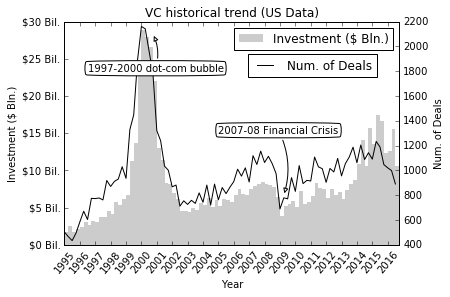
\includegraphics[scale=0.9]{vc_trend_2}
    \caption{ \textbf{VC investment trend in US}\\Source: \parencite[][]{moneytree}, graph by author}
    \label{fig:vc_trend}
\end{figure}

%%%%%%%%%%%%%%%%%%%%%%%%%%%%%%%%%%%%%%%%
%%%%       NEW SECTION              %%%%
%%%%%%%%%%%%%%%%%%%%%%%%%%%%%%%%%%%%%%%%
\section{Aims and objectives of the research}
The aim of the research is to determine the effect of Venture Capital on the success of startups.

The research will to develop a model determining the effect of the Venture Capital on financial performance of Startups in the USA. Within the research we will construct the econometric model determining regression dependence of startups' performance indicators and Venture Capital invested in startups.

The \underline{sub-objectives} seek to answer the following questions:
\begin{enumerate}
    \item what are parameters that determine the development of startups?
    \item what internal factors are of great importance for developing the startups?
    \item what should be parameters of the model developed in the Thesis in order to determine the regression dependence of startups performance indicators and Venture Capital invested in startups?
    \item is the determined model suitable for the USA?
\end{enumerate}


For carrying out the analysis two selections representing annual data across the USA from 2000 for 2015 were created. The selection is based on availability of statistical data concerning amounts of VC transactions in the USA. 
%All data were nominated in millions of US dollars in real terms of 2005.
The following sources were considered for the research:

\begin{itemize}
    \item Bureau of the economic analysis of the USA (BEA)
    \item Organizations for Economic Cooperation and Development (OECD)
    \item The World Bank (WB)
    \item The World Trade Organization (WTO)
    \item Administration on development of small business of the USA (SBA)
    \item World Intellectual Property Organization (WIPO)
    \item National association of venture capital of the USA
\end{itemize}

In accordance with the objectives of the study the following hypotheses are put forward:
\begin{enumerate}
    \item Venture Capital is of great importance for developing the startups
    \item Venture Capital positively influences the financial performance of the startups
\end{enumerate}
Finally, the research will be based on the author’s individual professional point of view and every approach will be explained.


